% !TeX spellcheck = ru_RU
% !TEX root = vkr.tex

\section{Обзор предметной области}

В данном разделе представлен обзор некоторых существующих методов и концепций, связанных с графами. В частности, используемая терминология, способы представление разреженных структур, алгоритм обхода графа в ширину и параллельные вычисления.

\subsection{Терминология}

\newtheorem{definition}{Определение}
\newtheorem*{remark}{Замечание}

\begin{definition}
Простой неориентированный граф $\mathcal{G}$ --- это упорядоченная пара конечных множеств $V$ и $E$ таких, что $\mathcal{G} = \langle V, E \rangle$, $V$ --- непустое множество, элементы которого называются вершинами, и $E$ --- множество неупорядоченных пар вершин, называемых рёбрами.
\end{definition}

\begin{definition}
Простой ориентированный граф $\mathcal{G}$ --- это упорядоченная пара  конечных множеств $V$ и $E$ таких, что $\mathcal{G} = \langle V, E \rangle$,  $V$ --- непустое конечное множество, элементы которого называются вершинами, и $E \subseteq V \times V$ --- множество упорядоченных пар вершин, называемых рёбрами.
\end{definition}

\begin{definition}
Помеченный ориентированный граф --- это упорядоченная пара $\langle \mathcal{G}, \mu \rangle$, где $\mathcal{G}$ --- простой ориентированный граф, и отображение $\mu: E \rightarrow L$, сопоставляющее каждому ребру $e \in E$ метку (вес) из множества~$L$. Помеченный неориентированный граф определяется аналогично.
\end{definition}

\begin{definition}
Весовая матрица графа $\mathcal{G}$ --- это квадратная матрица $A = (a_{ij})$ порядка $n$, где $n$ --- количество вершин графа $\mathcal{G}$, а элемент $a_{ij}$ равен весу ребра, соединяющего вершины $i$ и $j$, или значению, указывающему на его отсутствие.
\end{definition}

\begin{definition}
Матрица смежности графа $\mathcal{G}$ --- это квадратная матрица $A = (a_{ij})$ порядка $n$, где $n$ --- количество вершин графа $\mathcal{G}$, а элемент $a_{ij}$ равен 1, если между вершинами $i$ и $j$ есть ребро, или 0, если ребра нет.
\end{definition}

\begin{remark}
Для удобства под матрицей смежности ориентированного графа иногда подразумевают весовую, принимая вес между вершинами за 1, а значение, указывающее на отсутствие ребра, за 0.     
\end{remark}

\begin{definition}
Структура данных дерево --- это иерархическая структура данных, представляющая набор связанных элементов --- узлов. В каждом дереве существует ровно один корневой узел, имеющий от 0 до $n$ узлов-потомков (которые аналогично имеют от 0 до $n$ потомков) и ни одного узла-предка. А также конечное число узлов, не имеющих ни одного потомка, называемых листьями.
\end{definition}

\begin{definition}
Бинарное дерево --- это дерево, каждый узел которого, за исключением листьев, имеет от 0 до 2 узлов-потомков.
\end{definition}

\subsection{Представление разреженных структур}

Ниже представлены несколько существующих форматов хранения разре\-жен\-ных матриц.

\textit{Наивный} способ представления разреженных структур предполагает хранение всех элементов, включая нулевые, указывающие на отсутствие связей или отношений. Этот подход требует больших затрат памяти и на практике малоэффективен.

\textit{Координатное представление} (\textit{COO}) использует тройки ($i$, $j$, $value$) для представления ненулевых элементов разреженной структуры. Параметры ($i$, $j$) указывают на позицию элемента в матрице, а $value$ --- на его значение. На практике используют три неупорядоченных массива (один для каждой координаты тройки) и скаляр, отвечающий за общее количество непустых ячеек \cite{stanimirovic2009performance}. Такая модель используется для хранения небольших разреженных структур и может быть неэффективна при работе с большими данными. В частности, из-за необходимости перебора большого количества троек при поиске, и трудностей с добавлением новых элементов.

Форматы хранения \textit{Compressed Sparse Row} (\textit{CSR}) и \textit{Compressed Spar\-se Column} (\textit{CSC}) не основаны на конкретном свойстве
и могут быть использованы для хранения любой разреженной матрицы \cite{stanimirovic2009performance}. Исходные данные распределяются на несколько массивов --- один, содержащий значения ненулевых элементов, один для хранения индексов строк или столбцов (в CSR по строкам, а в CSC по столбцам) соответствующих элементов и один массив-указатель на первое ненулевое вхождение каждой строки или столбца. Аналогично координатному формату вставка или удаление элементов в CSR/CSC может потребовать перестройки всей структуры. Кроме того, в них сложнее обеспечить эффективное параллельное выполнение операций \cite{bulucc2009parallel}.

\textit{Дерево квадрантов} (Quadtree) --- это структура данных, часто используемая для представления разреженных двумерных данных. Quad\-tree разбивается на четыре части (реже на любое другое количество частей), называемых \textit{квадрантами}, где каждый квадрант может быть разбит на четыре подквадранта и т.~д. Если в одной области наблюдаются только элементы одного типа (например, нули в разреженных матрицах), дерево \enquote{обрезают} до одного листа, содержащего информацию об узлах, расположенных на нижних уровнях. Из-за своей рекуррентной природы дерево квадрантов удобно использовать для параллельных вычислений.

\subsection{Алгоритм обхода графа в ширину}

Ниже приведено неформальное описание работы BFS.

\begin{enumerate}
    \item Инициализировать очередь --- структуру данных для хранения вершин, которые необходимо посетить --- и пустой массив для хранения посещённых вершин. Добавить вершины, с которых начинается поиск, в очередь.
    \item Удалить первую вершину из очереди. Пометить эту вершину как посещённую.
    \item Добавить вершины, соединённые ребром с текущей, в очередь.
    \item Повторить пункты 2--3, пока очередь не окажется пустой.
\end{enumerate}

\begin{figure}
    \centering
    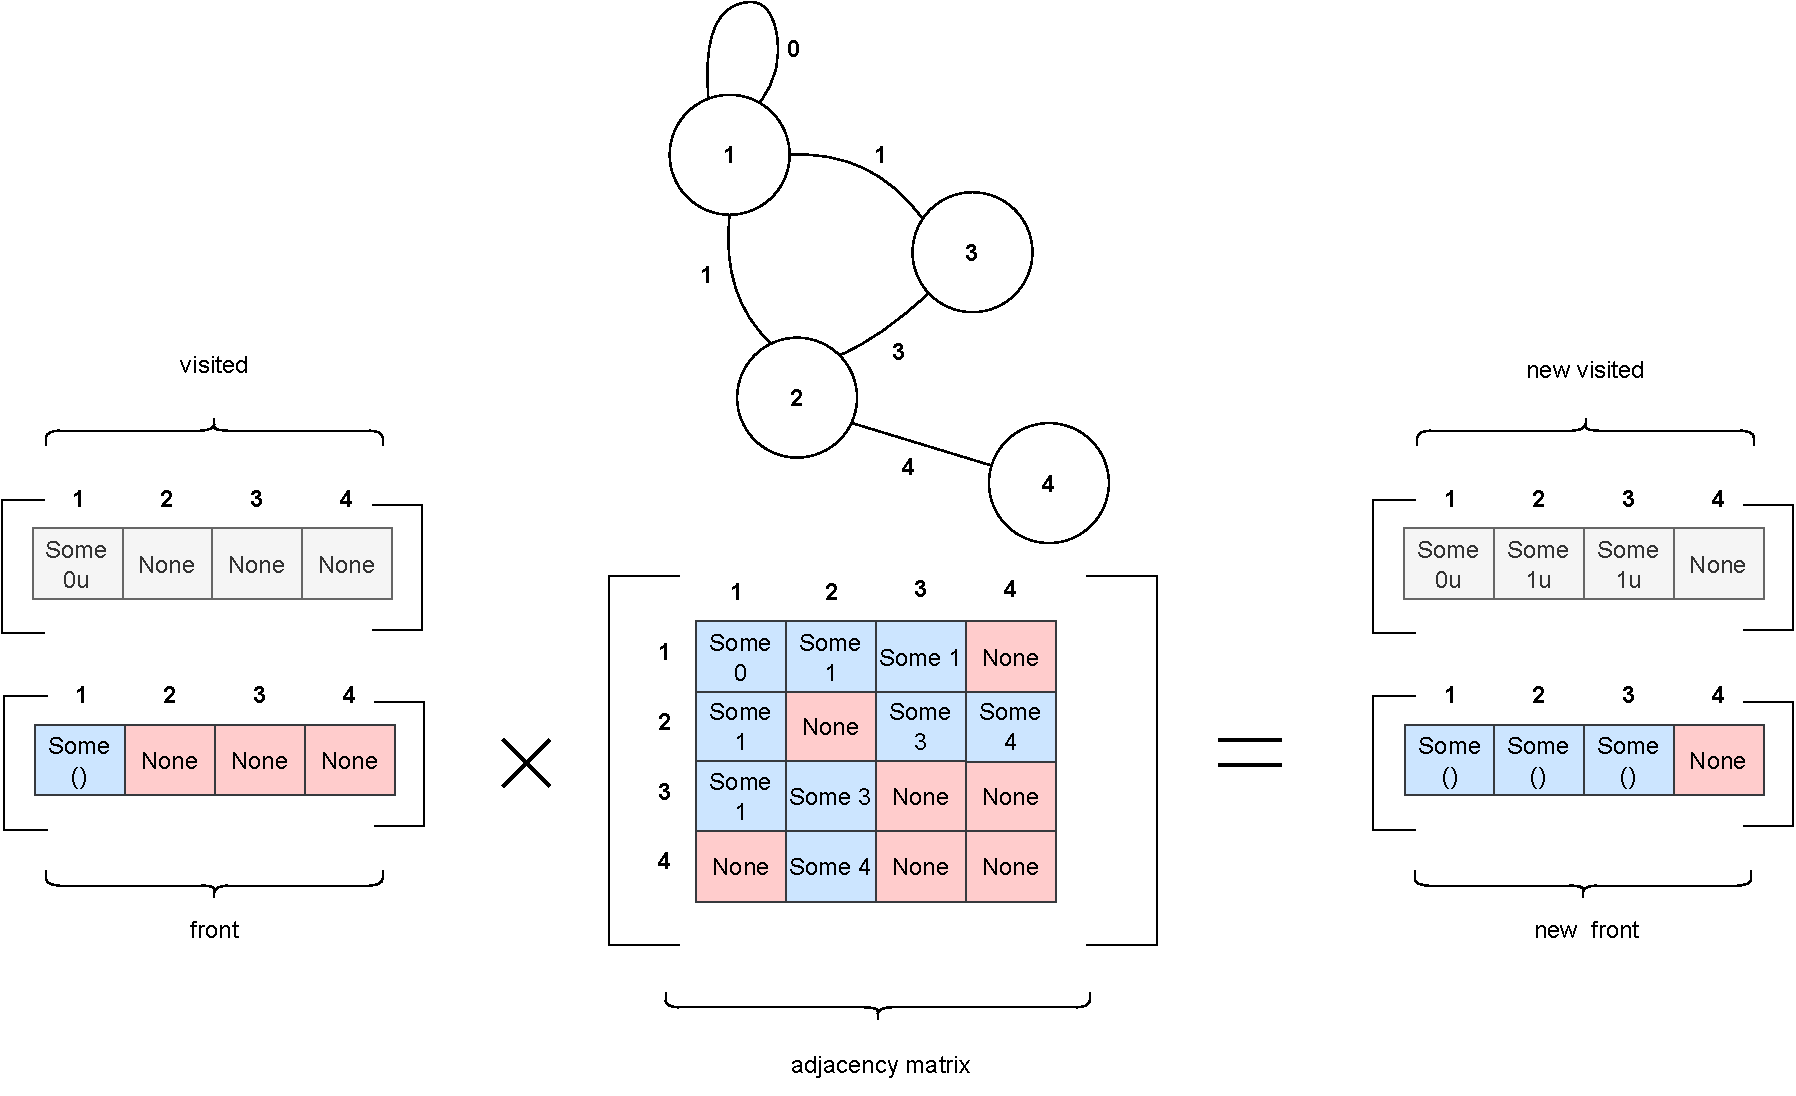
\includegraphics[width=\textwidth]{BFSLinearAlgebra.pdf}
    \caption{Шаги 3--4 BFS с использованием линейной алгебры}
    \label{fig:bfs}
\end{figure}

Как было упомянуто раннее, линейная алгебра может быть полезна при реализации некоторых этапов BFS, например, для эффективного представления графа или выполнения операций над матрицами и векторами внутри алгоритма. Ниже приведена реализация шагов 1--4 с использованием векторно-матричных операций.

\begin{enumerate}
    \item Инициализировать матрицу смежности графа (\texttt{ad\-ja\-cen\-cy mat\-rix}), вектор для хранения посещённых вершин (\texttt{visited}) и вектор схожий с очередью, называемый фронтом (\texttt{front}), в котором хранятся вершины, находящиеся на текущем уровне обхода. Добавить вершины, с которых начинается поиск, в \texttt{visited}.
    \item Умножить \texttt{front} на \texttt{adjacency matrix} и получить новый фронт  (\texttt{new front}), добавив, таким образом, все вершины, соединённые с текущей. 
    \item Сложить \texttt{new front} с \texttt{visited} и получить новый вектор (\texttt{mask}) так, что значения из нового фронта сохраняются, только когда они не были помечены в \texttt{visited} (это действие избавит нас от многократного посещения одной и той же вершины). Обновить \texttt{visited} (\texttt{new visited}), используя полученный вектор и векторные операции.
    \item Повторить шаги 2--3, пока все вершины не будут помечены как посещённые.
\end{enumerate}

На рис. \ref{fig:bfs} представлен пример работы алгоритма обхода графа в ширину с использованием линейной алгебры.

\subsection{Параллельные вычисления и многопоточность}

Большинство несложных программ с большой вероятностью выполняются в одном \textit{потоке}. Другими словами, в любой момент времени только один оператор находится в процессе выполнения; и если поток блокируется, то вся работа программы останавливается \cite{sarcar2022threading}.

Использование \textit{ядер} центрального процессора может уменьшить общее время простоя и повысить эффективность программы. Как правило, одно ядро за раз обслуживает только один поток. Однако, даже процессор одноядерной машины, быстро переключаясь между задачами, способен создавать иллюзию их одновременного выполнения. В связи с этим, когда несколько потоков, работающих на одном ядре, могут \enquote{чередоваться}, эффективнее использовать больше потоков, чем имеющихся ядер \cite{Lee2020}.

При реализации многопоточности, стоит обратить внимание на следующие особенности.
\begin{enumerate}
    \item \textit{Накладные расходы на синхронизацию}. Во избежание некорректной работы при использовании нескольких потоков необходимо обеспечить их синхронизацию. Координация, в свою очередь, вызывает накладные расходы, что не лучшим образом влияет на производительность.
    \item \textit{Конкуренция за ресурсы}. Когда несколько потоков пытаются получить доступ к общим ресурсам, возникает конкуренция, замедляющая работу программы.
    \item \textit{Накладные расходы на создание}. Создание потоков и управление ими требуют дополнительных ресурсов.
    \item \textit{Зависимость от алгоритмов и данных}. Некоторые алгоритмы (данные) не могут быть эффективно распараллелены из-за своей природы.
    \item \textit{Зависимость от аппаратного обеспечения}. Некоторые системы имеют ограниченное количество доступных ядер, что оказывает влияние на возможности параллельных вычислений.
\end{enumerate}

Данные аспекты были учтены при проведении экспериментального исследования и анализе полученных результатов.